\section{Experiments Setting Details}\label{app:exp-details}

\paragraph{Backbone Models.} Although powerful models such as GPT-4 exhibit notable robustness to adversarial interference, smaller and less sophisticated models remain highly vulnerable, experiencing significant accuracy drop under adversarial conditions. To effectively assess the robustness and efficiency of our proposed framework, we select lightweight open-source models as the backbone for both individual agents and the coordinator. Lightweight models offer the advantage of resource-efficient loading and execution, thus ensuring scalability and practicality in multi-agent settings. Specifically, we employ LLaMA 3.2 (3B)~\cite{llama3.2}, Mistral (7B)~\cite{mistral7b}, and Qwen2.5 (7B)~\cite{qwen2.5} as our backbone models.
Moreover, we utilize GPT-4o mini~\cite{gpt4o-mini} as an external judge to assess the quality and correctness of the final responses generated by the multi-agent team.


\paragraph{Datasets.} We evaluate the effectiveness of our proposed framework across five benchmark datasets: MMLU~\cite{MMLU}, MATH~\cite{math}, GSM8K~\cite{gsm8k}, HumanEval~\cite{humaneval}, and Research Questions~\cite{researchQA}. Specifically, we use high school mathematics and statistics questions from the MMLU dataset, which are referred to as MMLU-MS, to assess the performance of the model in multiple-choice question answering. The MATH and GSM8K datasets are employed to evaluate mathematical reasoning capabilities, while HumanEval is used to assess coding proficiency. The Researchy Questions dataset consists of non-factoid questions derived from real-world search engine queries, characterized by their subjective nature and absence of a singularly correct answer. In this context, a human judge or an external judge must carefully evaluate agent responses, determining correctness based on provided instructions and contextual information. 

\subsection{Collaboration Setup}

Our primary experiments involve a team of five agents, comprising two faithful agents and three adversarial agents explicitly instructed to introduce subtle inaccuracies in their responses without revealing their adversarial nature. We employ consistent prompts across various tasks, adapting only the task-specific details. Our analysis primarily explores two main communication structures: a Stochastic Interaction  Architecture (SIA) , Standalone Agent Architecture (SAA) and a Credibility-ordered Chain. 



\subsubsection{Standalone Agent Architecture (SAA)}

In SAA every agent receives the same question $Q$ and produces an answer \emph{without any communication}.  
The resulting communication graph is edgeless: $G=(\mathcal{A},\emptyset)$.
We aggregate the set of agent answers $R=\{x_1,\dots,x_{|R|}\}$ using the centroid-based ensemble method of \cite{requal}.  
Let $v(x)$ be the embedding of answer $x$ and let $w_i\propto\operatorname{CrS}^{(i)}$ be the credibility weight of agent~$i$.  
The credibility‑weighted centroid is  
\[
\mathbf{v}_c=\frac{1}{|R|}\sum_{i=1}^{|R|} w_i\,\mathbf{v}(x_i),
\]  
and the final answer is the one whose embedding is closest (cosine distance $d$) to that centroid:  
\[
x^\star=\arg\min_{x\in R} d\!\bigl(\mathbf{v}(x),\mathbf{v}_c\bigr).
\]  
Finally, we calculate each agent’s Contribution Score (CSc)—derived from the Shapley value as described in\S\ref{sec:tech-details-Csc}—and, from these, obtain the Credibility Scores (CrS) for the entire set of responses.


\subsubsection{Stochastic Interaction Architecture (SIA)}
SIA adds a sparse, random communication graph $G_t$ that is resampled for every query.  
For each question we draw $m$ undirected edges from the $\binom{N}{2}$ possible pairs with replacment ($N= 5, m=6$ in our experiments), typically creating six links.  
Connected agents exchange their current answers and may revise them, producing diverse topologies such as trees, rings, and other sparse structures—while avoiding full information saturation that would otherwise aid adversaries.


\subsubsection{Credibility-ordered Chain}
To further test our hypothesis within a specific, stable structure, we introduce the chain-based architecture. 
In the chain architecture agents are sorted in descending order of their credibility score in the beginning of the experiment. Communication in this structure only occurs between adjacent agents. 
Positioning the most reliable agents earlier in the chain limits the influence of adversaries further down the chain. Although the communication pattern remains fixed, CrS values continue to be updated throughout the interactions within the chain.

% In this architecture, agents are sorted based on their credibility scores (CrS) in descending order, positioning  agents earlier in the chain to reduce the impact of adversaries on the team. 

\subsection{Why Three Architectures?}
SAA provides a lower bound on performance—no interactions means no adversarial persuasion—while SIA explores the hard regime where adversaries may form majorities and hijack discussions by persuading other agents. The credibility‑ordered chain tests our hypothesis in a stable yet asymmetric structure. Experiments in \S\ref{sec:experiments} demonstrate that CSc/CrS significantly improve robustness across all three settings.

\section{Extended Experiment Results}\label{app:exp-ext}


\subsection{Judge Alters the Outcome}

The effectiveness of the judge is highly task-dependent. To illustrate this, we present results on two different benchmarks: HumanEval for code completion, and GSM8K for mathematical reasoning.

On the HumanEval benchmark, using GPT-4o mini as the judge proves problematic. In this task, the judge receives a reference solution, a set of test functions, and the final response generated by the CrS coordinator. However, it often fails to correctly determine whether the generated code is functionally correct. This results in numerous cases where incorrect solutions are mistakenly rewarded with a score of 1, severely distorting the Contribution Scores (CSc) and, consequently, the Credibility Scores (CrS). As shown in Table~\ref{tab:humaneval_comp}, these misjudgments ultimately hurt overall system accuracy.

For mathematical reasoning questions from GSM8K, we observe a different failure mode when using a weaker judge. Figure~\ref{fig:llama-judge} shows the CrS trajectories for five agents—two faithful and three adversarial—when LLaMA 3.2's is used as the evaluator. Compared to the more stable CrS patterns seen with GPT-4o mini (Figure~\ref{fig:judge-weight}), the scores here fluctuate significantly. This instability stems from LLaMA 3.2's tendency to produce malformed outputs or to incorrectly assess agent contributions—such as returning a two-element array (e.g., $[0.2, 0.8]$) in a five-agent setting—indicating its limited ability to follow contribution-scoring instructions accurately.  



\definecolor{softyellow}{RGB}{255, 249, 196}
\definecolor{softblue}{RGB}{226, 240, 255}


\begin{table*}[h!]
\centering
\small
\setlength{\tabcolsep}{4.5pt}
\renewcommand{\arraystretch}{1.1}
\begin{tabular}{lccccccp{2.8cm}c}
\toprule
\textbf{Agent} & L1 & L2 & L3 & L4 & L5 & L6 & \textbf{CrS (curr→fut.)} & \textbf{CSc} \\
\midrule
Agent 1: B & \cellcolor{softyellow}B & B & B & \cellcolor{softyellow}X & X & X & $0.4593 \rightarrow 0.4617$ & 0.15 \\
Agent 2: B & B & \cellcolor{softyellow}B & \cellcolor{softyellow}D & D & \cellcolor{softyellow}C & C & $0.4143 \rightarrow 0.4143$ & 0.20 \\
Agent 3: B & B & B & B & B & \cellcolor{softyellow}B & \cellcolor{softyellow}D & $0.4224 \rightarrow 0.4225$ & 0.20 \\
Agent 4: B & B & \cellcolor{softyellow}C & \cellcolor{softyellow}X & \cellcolor{softyellow}C & C & \cellcolor{softyellow}D & $0.4711 \rightarrow 0.4688$ & 0.25 \\
Agent 5: C & \cellcolor{softyellow}C & C & C & C & C & C & $0.4655 \rightarrow 0.4656$ & 0.20 \\
\midrule
\rowcolor{softblue}
\multicolumn{7}{r}{\textbf{Final Answer}} & C & \\
\rowcolor{softblue}
\multicolumn{7}{r}{\textbf{Correct Answer}} & D & \\
\rowcolor{softblue}
\multicolumn{7}{r}{\textbf{Reward}} & -1 & \\
\bottomrule
\end{tabular}
\caption{Compact illustration of agent response dynamics and credibility updates. Yellow cells indicate response changes.}
\label{tab:example-table-1}
\end{table*}









% \begin{table}[h!]
% \centering
% \resizebox{0.9\columnwidth}{!}{%
% \begin{tabular}{lcc|cc}
% \toprule
% $pass@k, k=1$ & \multicolumn{2}{c}{Pre-Communication} & \multicolumn{2}{c}{Post-Communication} \\ 
% \cmidrule(lr){2-3} \cmidrule(lr){4-5}
% Approach & Chain & Random & Chain & Random \\ 
% \midrule
% CrS-based Coord. & - & X & $0.16$& $0.12$ \\ 
% Simple Coord.    & - & X & $0.08$ &X \\ 
% Llama 3.2        & $0.01$ & X & $0.14$&$0.10$ \\ 
% \bottomrule
% \end{tabular}%
% }
% \caption{Comparison of accuracies before and after communication on a sample of 50 questions from HumanEval dataset.}
% \label{tab:methods_comp}
% \end{table}



% \begin{table}[h!]
% \centering
% \resizebox{0.9\columnwidth}{!}{%
% \begin{tabular}{lcc|cc}
% \toprule
%  & \multicolumn{2}{c}{Pre-Communication} & \multicolumn{2}{c}{Post-Communication} \\ 
% \cmidrule(lr){2-3} \cmidrule(lr){4-5}
% Approach & Chain & Random & Chain & Random \\ 
% \midrule
% CrS-based Coord. & - & X & $0.16$& $0.12$ \\ 
% Simple Coord.    & - & X & $0.08$ &X \\ 
% Llama 3.2        & $0.01$ & X & $0.14$&$0.10$ \\ 
% \bottomrule
% \end{tabular}%
% }
% \caption{Comparison of accuracies before and after communication on a sample of 50 questions from HumanEval dataset.}
% \label{tab:methods_comp}
% \end{table}


% labels = ['Llama3.2 - Aggregator Agent','Llama3.2 - Single Agent', 'CrS-based Llama3.2 Coordinator - Multi Agent', 'Llama3.2 Majority Voting - Multi Agent']
% [[0.15, 0.4, 0.29, 0.22],
%  [0.1, 0.41, 0.33, 0.23],
%  [0.09980806142034548, 0.29558541266794625, 0.18809980806142035, 0.1],
%  [0.08, 0.3, 0.3, 0.3]]

% labels =['Llama3.2 - Single Agent', 'CrS-based Llama3.2 Coordinator - Multi Agent', 'Llama3.2 Majority Voting - Multi Agent', 'Llama3.2 - Similarity Ensemble']

% [[0.12, 0.29, 0.2, 0.16],
%  [0.16, 0.33, 0.21, 0.13],

%  [0.11900191938579655,
%   0.2802303262955854,
%   0.1727447216890595,
%   0.1324376199616123],
  
%  [0.18098159509202455,
%   0.3312883435582822,
%   0.2392638036809816,
%   0.17177914110429449]]





\definecolor{softyellow}{RGB}{255, 249, 196}
\definecolor{softblue}{RGB}{226, 240, 255}

\begin{table*}[h!]
\centering
\small
\setlength{\tabcolsep}{4.5pt}
\renewcommand{\arraystretch}{1.1}
\begin{tabular}{lccccccp{2.8cm}c}
\toprule
\textbf{Agent} & L1 & L2 & L3 & L4 & L5 & L6 & \textbf{CrS (→)} & \textbf{CSc} \\
\midrule
Agent 1: D & \cellcolor{softyellow}B & B & B & B & B & \cellcolor{softyellow}A & $0.4841 \rightarrow 0.4940$ & 0.00 \\
Agent 2: B & \cellcolor{softyellow}X & X & \cellcolor{softyellow}A & A & A & A & $0.3613 \rightarrow 0.3686$ & 0.00 \\
Agent 3: B & B & B & B & \cellcolor{softyellow}X & X & X & $0.4034 \rightarrow 0.3951$ & 0.40 \\
Agent 4: B & B & \cellcolor{softyellow}A & \cellcolor{softyellow}A & \cellcolor{softyellow}C & \cellcolor{softyellow}A & \cellcolor{softyellow}C & $0.4561 \rightarrow 0.4468$ & 0.40 \\
Agent 5: C & C & \cellcolor{softyellow}C & C & C & \cellcolor{softyellow}C & C & $0.5139 \rightarrow 0.5139$ & 0.20 \\
\midrule
\rowcolor{softblue}
\multicolumn{7}{r}{\textbf{Final Answer}} & C & \\
\rowcolor{softblue}
\multicolumn{7}{r}{\textbf{Correct Answer}} & B & \\
\rowcolor{softblue}
\multicolumn{7}{r}{\textbf{Reward}} & -1 & \\
\bottomrule
\end{tabular}
\vspace{0.5em}
\caption{Illustrative example from MMLU with two faithful agents. Although the final response was incorrect, these agents were not penalized— the judge identified adversarial influence from Agent 4 based on the communication history.}
\label{tab:highlighted_table}
\end{table*}




 \begin{figure}[ht]
    % \centering
    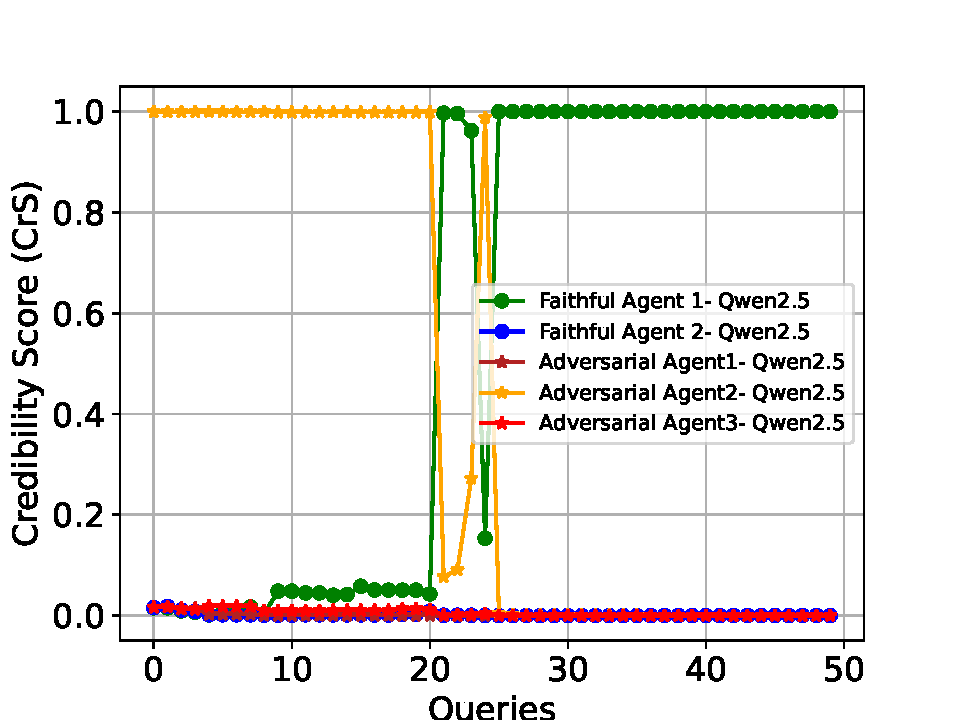
\includegraphics[width=0.5\textwidth]{plots/newjudge_weights_qwen2.5-2.pdf}
    \caption{CrS evolution with a LLaMA‑3.2(3B) judge supervising five Qwen2.5(7B) agents on GSM8K—directly comparable to Figure\ref{fig:judge-weight-a}. }
    \label{fig:llama-judge}
\end{figure}


\begin{figure*}[t]              
  \centering
  \begin{subfigure}[b]{0.46\textwidth}
    \centering
    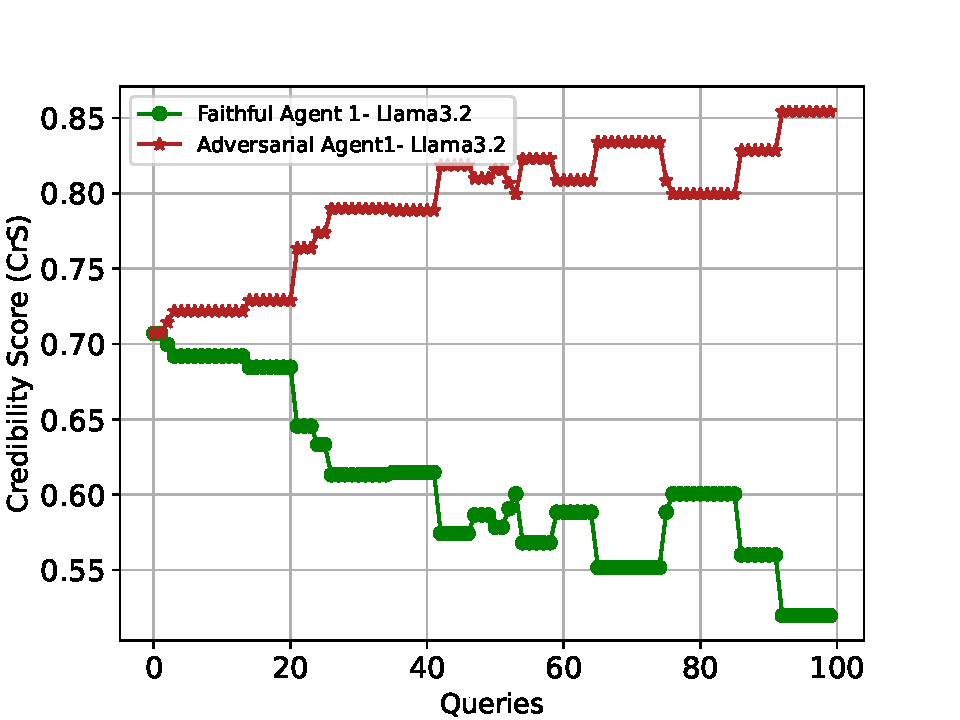
\includegraphics[width=\linewidth]{plots/2agents_1ad_weights_gsm8k_connected.pdf}
    \caption{After exchanging messages, Each agent outputs a revised solution, and an identical LLaMA‑3.2 coordinator produces the final response using CrS‑weighted aggregation of their answers.}
    \label{crs-saa}
  \end{subfigure}%
  \hfill
  \begin{subfigure}[b]{0.46\textwidth}
    \centering
    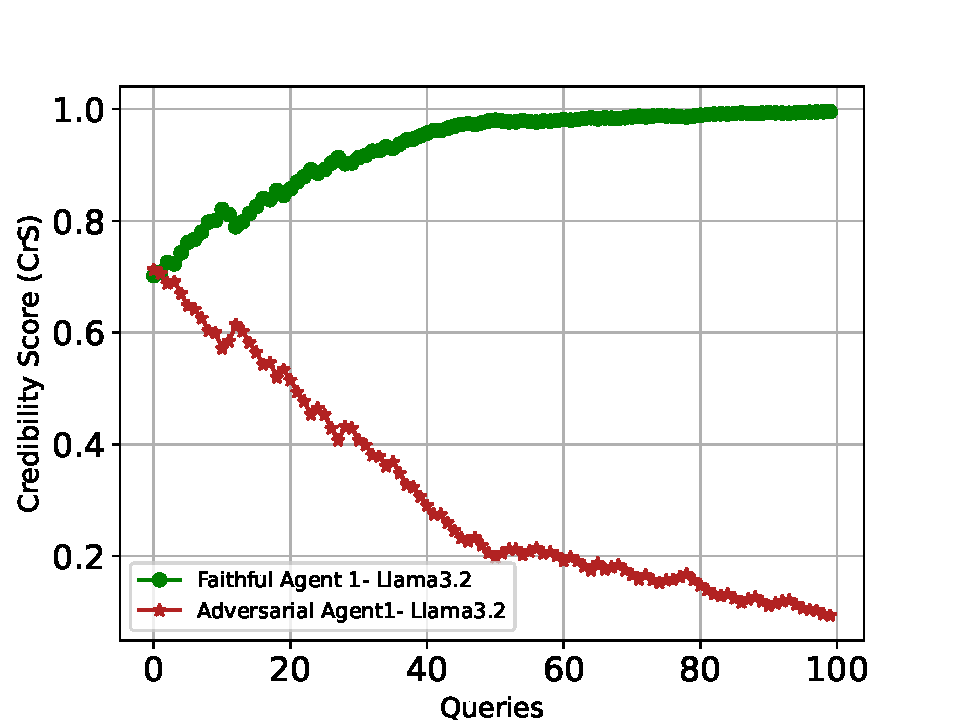
\includegraphics[width=\linewidth]{plots/2agents_1ad_weights_gsm8k.pdf}
    \caption{The agents have no inter‑agent communication (SAA). Each agent generates a candidate answer, and the coordination mechanism selects the answer nearest to their CrS‑weighted centroid.}
    \label{crs-sia}
  \end{subfigure}

  \vspace{0.5em}  
  \caption{CrS evolution for two independent LLaMA‑3.2 (3B).}
  \label{Crs-Shapley}
\end{figure*}



% \input{diagram}
% \begin{figure*}[t]
%     \centering
%     \includegraphics[width=\textwidth]{diagrams/process-diagram.pdf}
%     \caption{}
%     \label{fig:proc-diagram}
% \end{figure*}

